\section{实验四:Traps}\label{sec:Traps}

通过中断实现系统调用

\subsection{实验目的}

\begin{enumerate}
	\item 进一步了解系统调用所发挥的重要作用。
	\item 掌握通过中断进行系统调用的过程及其所发挥的作用。
	\item 了解简单的汇编语言,知道汇编语言是如何发挥作用的。
	\item 理解 xv6 中的堆栈,同时试着实现一个用户级中断处理。
\end{enumerate}

\subsection{实验内容}

\begin{enumerate}
	\item 了解 RISC-V 程序集,阅读 call.asm 中的函数 g、f 和 main 的代码,并回答问题。
	\item 完成 Backtrace 函数,当发生错误的时候查看当前堆栈中的系统调用。
	\item 添加系统调用 sigalarm,当用户程序运行了 n 个 ticks 后,触发回调函数。
\end{enumerate}

\subsection{实验准备}

\begin{enumerate}
	\item 阅读 xv6 参考书的第 4 章。
	\item 阅读从用户空间切换到内核空间并返回涉及的程序集 \texttt{kernel/trampoline.S}。
	\item 阅读处理中断的代码 \texttt{kernel/trap.c}。
\end{enumerate}

\subsubsection{RISC-V 寄存器}

RISC-V 有 32 个通用寄存器和 32 个浮点寄存器。详细信息如\cref{tab:riscv-regs} 所示。

\begin{table}[!hpt]
	\caption{RISC-V 寄存器说明}
	\label{tab:riscv-regs}
	\centering
	\begin{tabular}{@{}cclc@{}} \toprule
		\textbf{编号} & \textbf{别名} & \textbf{作用说明} & \textbf{保存者} \\
		\midrule
		x0  & zero     & 恒为0,不能被修改                  & --      \\
		x1  & ra       & 返回地址(Return Address)         & Caller  \\
		x2  & sp       & 栈指针(Stack Pointer)            & Callee  \\
		x3  & gp       & 全局指针(Global Pointer)         & --      \\
		x4  & tp       & 线程指针(Thread Pointer)         & --      \\
		x5--x7   & t0--t2    & 临时寄存器(Temporaries)          & Caller  \\
		x8  & s0/fp    & 保存/帧指针(Saved/Frame Pointer) & Callee  \\
		x9  & s1       & 保存寄存器(Saved)                & Callee  \\
		x10--x11 & a0--a1    & 函数参数/返回值(Arg/Ret)             & Caller  \\
		x12--x17 & a2--a7    & 函数参数(Arg)                        & Caller  \\
		x18--x27 & s2--s11   & 保存寄存器(Saved)                & Callee  \\
		x28--x31 & t3--t6    & 临时寄存器(Temporaries)          & Caller  \\
		\midrule
		f0--f7   & ft0--ft7  & 浮点临时寄存器(FP Temporaries)   & Caller  \\
		f8--f9   & fs0--fs1  & 浮点保存寄存器(FP Saved)         & Callee  \\
		f10--f11 & fa0--fa1  & 浮点参数/返回值(FP Arg/Ret)      & Caller  \\
		f12--f17 & fa2--fa7  & 浮点参数(FP Arg)                 & Caller  \\
		f18--f27 & fs2--fs11 & 浮点保存寄存器(FP Saved)         & Callee  \\
		f28--f31 & ft8--ft11 & 浮点临时寄存器(FP Temporaries)   & Caller  \\
		\bottomrule
	\end{tabular}
\end{table}

保存者的意义:

\begin{enumerate}
	\item Caller:如果函数需要使用这些寄存器,则调用别的函数前要先保存它们的值,回来后再恢复。
	\item Callee:如果函数需要使用这些寄存器,进入函数前要先保存,用完后恢复,保证调用者的数据不被破坏。
\end{enumerate}

此外,还有一些特殊的寄存器:

\begin{enumerate}
	\item \texttt{stvec}:内核将其 trap 处理程序的地址写入此处;RISC-V 跳转到 \texttt{stvec} 中的地址来处理 trap。
	\item \texttt{sepc}:当trap发生时,RISC-V将程序计数器保存在这里(因为 \texttt{pc} 随后会被 \texttt{stvec} 中的值覆盖)。\texttt{sret}(从trap返回)指令将 \texttt{sepc} 复制到 \texttt{pc}。内核可以编写 \texttt{sepc} 来控制 \texttt{sret} 的去向
	\item \texttt{scause} :RISC-V 在此处放置一个数字来描述 trap 的原因。
	\item \texttt{sscratch} :trap 处理程序代码使用 \texttt{scratch} 来帮助避免在保存用户寄存器之前覆盖它们。
	\item \texttt{sstatus}:\texttt{sstatus} 中的SIE位控制是否启用设备中断。如果内核清除SIE,RISC-V 将推迟设备中断,直到内核设置SIE。SPP位指示trap是来自用户模式还是管理模式,并控制 \texttt{sret} 返回的模式。
\end{enumerate}

\subsubsection{RISC-V 中断机制}

上述寄存器与管理模式下处理的trap相关,并且不能在用户模式下读取或写入。对于机器模式下处理的trap,有一组类似的控制寄存器;xv6仅将它们用于定时器中断的特殊情况。

当需要强制trap时,RISC-V硬件会对所有trap类型(定时器中断除外)执行以下操作:

\begin{enumerate}
	\item 如果trap是设备中断,并且\texttt{sstatus} SIE位清零,则不要执行以下任何操作。
	\item 通过清除\texttt{sstatus} 中的SIE位来禁用中断。
	\item 将 \texttt{pc} 复制到 \texttt{sepc}。
	\item 将当前模式(用户或管理)保存在 \texttt{sstatus} 的SPP位中。
	\item 设置 \texttt{scause} 以反映 trap 的原因。
	\item 将模式设置为管理模式。
	\item 将 \texttt{stvec} 的值复制到pc
	\item 开始执行 \texttt{pc} 指向的trap handler的代码
\end{enumerate}

\subsubsection{常见汇编指令}

\begin{enumerate}
	
	\item 数据传送指令:
	
	\texttt{li reg, imm}:将立即数 imm 加载到 reg。
	
	\texttt{mv reg1, reg2}:reg1 = reg2。
	
	\texttt{ld reg, offset(base)}:从内存 base+offset 读 8 字节到 reg。
	
	\texttt{sd reg, offset(base)}:将 reg 的值写到 base+offset 的内存。
	
	\item 算术/逻辑运算指令:
	
	\texttt{addi reg1, reg2, imm}:reg1 = reg2 + imm。
	
	\texttt{add reg1, reg2, reg3}:reg1 = reg2 + reg3。
	
	\texttt{sub reg1, reg2, reg3}:reg1 = reg2 - reg3。
	
	\texttt{and/or/xor reg1, reg2, reg3}:位运算(且/或/异或)。
	
	\item 跳转/分支指令:
	
	\texttt{jalr rd, rs1, imm}:跳转到 rs1+imm,并把返回地址(当前PC+4)存到 rd。
	
	\texttt{jal reg, offset}:跳转并保存返回地址到 reg。
	
	\texttt{jr reg}:跳转到 reg 指向的地址。
	
	\texttt{beq reg1, reg2, offset}:相等跳转。
	
	\texttt{bne reg1, reg2, offset}:不等跳转
	
	\item 控制寄存器操作指令:
	
	\texttt{csrw csr, reg}:将 reg 的值写入控制状态寄存器 csr。
	
	\texttt{csrr reg, csr}:将 csr 的值读到 reg。
	
	\texttt{csrrw reg1, csr, reg2}:reg1 \textless-\textgreater{} csr 交换。
	
	\item 特殊指令:
	
	\texttt{sfence.vma zero, zero}:刷新 TLB(页表切换后要用)。
	
	\texttt{sret}:从陷入(trap)返回用户态。
\end{enumerate}

\subsubsection{函数调用堆栈,函数调用栈帧}

函数调用堆栈(call stack)如\cref{fig:process_address_space} 的 stack 区域所示,是操作系统和编程语言运行时用来管理函数调用和返回的一种数据结构。它是内存中的一块区域,专门用来保存每次函数调用时的相关信息。

函数调用栈帧(stack frame)如\cref{fig:function_stack_frame} 所示,是指在程序执行过程中,每当一个函数被调用时,在调用堆栈上为该函数分配的一块内存区域。它用来保存该函数调用相关的信息,包括返回地址、上一级帧指针、局部变量、保存的寄存器等。函数调用栈帧是堆栈)上的基本单元。每次函数调用,都会在 stack 区域分配一个新的栈帧,保存该函数的运行环境。

xv6 中函数调用栈帧包含的内容有:

\begin{enumerate}
	\item return Address:函数返回时要跳转回的地址。
	\item To Prev. Frame (fp):上一级函数的帧指针(fp),用于回溯调用链。
	\item Saved Registers:被调用函数保存的寄存器。
	\item Local Variables:该函数的局部变量。
	\item fp(frame pointer):指向当前栈帧的顶部
	\item sp(stack pointer):指向当前栈顶(最低地址)
\end{enumerate}

其中,栈顶指针往下偏移 8 个字节是函数的返回地址,往下偏移 16 个字节是上一个栈帧的栈帧指针(previous frame pointer)。

\begin{figure}[!htb]
	\centering
	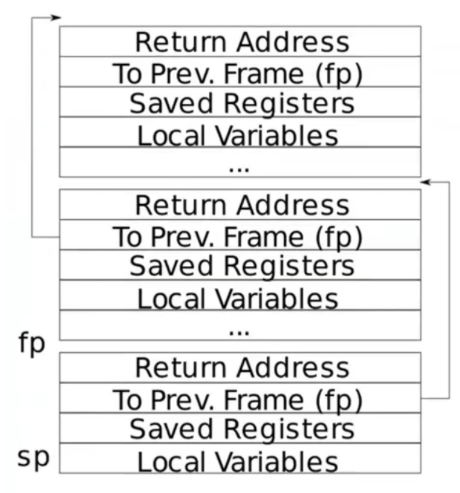
\includegraphics[width=0.6\textwidth]{function_stack_frame}
	\caption{函数调用栈帧}
	\label{fig:function_stack_frame}
\end{figure}

\subsubsection{来自用户空间的中断}

Xv6 对中断的处理方式有所不同,具体取决于中断是在内核中执行还是在用户代码中执行时发生。以下是来自用户代码的中断过程描述。

\paragraph{中断触发与入口}

\begin{itemize}
	\item 用户触发中断(\cref{lst:set_stvec})
	\begin{itemize}
		\item 用户程序在用户态运行,可能因为系统调用(如 ecall)、外部中断(如时钟中断)、异常(如非法访问)等原因,CPU 发生中断。
		\item RISC-V 硬件不会自动切换页表,trap 发生时仍在用户页表下。
	\end{itemize}
	\item PC 跳转到 uservec
	\begin{itemize}
		\item stvec 由 xv6 设置为 \texttt{TRAMPOLINE + (uservec - trampoline)},即 trampoline.S 中的 uservec。
		\item uservec 必须在用户页表和内核页表中都映射到同一虚拟地址(TRAMPOLINE,通常是最高虚拟地址 MAXVA)。
	\end{itemize}
\end{itemize}

\begin{listing}[!htb]
	\begin{minted}{c}
// trap.c: usertrapret()
w_stvec(TRAMPOLINE + (uservec - trampoline));
	\end{minted}
	\caption{将 stvec 设置为 uservec}\label{lst:set_stvec}
\end{listing}

\paragraph{uservec 处理}

\begin{itemize}
	\item 保存现场(\cref{lst:save_scene})
	\begin{itemize}
		\item uservec 开始时,所有的 32 个寄存器都是用户态的值,但是 uservec 需要对某些寄存器进行修改来设置satp,以便切换到内核页表。
		\item 先用 \texttt{csrrw a0, sscratch, a0} 交换 a0 和 sscratch,交换之前的sscratch中是指向user process的trapframe的地址,trapframe中预留了保存所有32个寄存器的空间。
		\item 使用 a0 把当前所有寄存器的值保存到 trapframe 中
	\end{itemize}
	\item 切换到内核页表并跳转(\cref{lst:switch_to_kernel_page_table} )
	\begin{itemize}
		\item 从 trapframe 读取内核页表地址,写入 satp,切换到内核页表。
		\item 读取 trapframe 中保存的 kernel stack、hartid、usertrap 地址等。
		\item 通过 jalr 跳转到 trapframe 里的 usertrap(kernel/trap.c)。
	\end{itemize}
\end{itemize}

\begin{listing}[!htb]
	\begin{minted}{gas}
# trampoline.S:21-30
uservec:    
        # swap a0 and sscratc
        # so that a0 is TRAPFRAME
        csrrw a0, sscratch, a0
        
        # save the user registers in TRAPFRAME
        sd ra, 40(a0)
        sd sp, 48(a0)
        # ... 保存其他寄存器
	\end{minted}
	\caption{保存现场}\label{lst:save_scene}
\end{listing}

\begin{listing}[!htb]
	\begin{minted}{gas}
# trampoline.S:70-80
        # restore kernel stack pointer from p->trapframe->kernel_sp
        ld sp, 8(a0)
        
        # make tp hold the current hartid, from p->trapframe->kernel_hartid
        ld tp, 32(a0)
        
        # load the address of usertrap(), p->trapframe->kernel_trap
        ld t0, 16(a0)
        
        # restore kernel page table from p->trapframe->kernel_satp
        ld t1, 0(a0)
        csrw satp, t1
        sfence.vma zero, zero
        
        # a0 is no longer valid, since the kernel page
        # table does not specially map p->tf.
        
        # jump to usertrap(), which does not return
        jr t0
	\end{minted}
	\caption{切换到内核页表并跳转}\label{lst:switch_to_kernel_page_table}
\end{listing}

\paragraph{usetrap 处理}

\begin{itemize}
	\item 检查中断发生的原因,确保来自用户态。
	\item 切换 stvec 为 kernelvec(内核态中断入口)。
	\item 保存 sepc(用户 PC)到 trapframe。
	\item 判断 trap 类型:
	\begin{itemize}
		\item 系统调用:调用 syscall(),epc+4 跳过 ecall。
		\item 设备中断:调用 devintr() 进行中断处理。
		\item 异常:打印信息,标记进程被杀死。
	\end{itemize}
	\item 检查进程是否被杀死,若被杀死则 exit 退出。
	\item 如果是时钟中断,yield() 让出 CPU。
	\item 调用 usertrapret() 返回用户态。
\end{itemize}

\begin{listing}[!htb]
	\begin{minted}{c}
// trap.c:37-90
void
usertrap(void)
{
    int which_dev = 0;

    if((r_sstatus() & SSTATUS_SPP) != 0)
        panic("usertrap: not from user mode");

    // send interrupts and exceptions to kerneltrap(),
    // since we're now in the kernel.
    w_stvec((uint64)kernelvec);
    
    struct proc *p = myproc();
    
    // save user program counter.
    p->trapframe->epc = r_sepc();

    if(r_scause() == 8){
        // system call
        if(p->killed)
            exit(-1);
        p->trapframe->epc += 4;
        intr_on();
        syscall();
    } else if((which_dev = devintr()) != 0){
         // ok
    } else {
        printf("usertrap(): unexpected scause %p pid=%d\n", r_scause(), p->pid);
        p->killed = 1;
    }

    if(p->killed)
        exit(-1);
    
    if(which_dev == 2)
    yield();
    
    usertrapret();
}
	\end{minted}
	\caption{函数 usertrap 的实现}\label{lst:usertrap}
\end{listing}

\paragraph{usetrapret 返回用户态}

\begin{itemize}
	\item 关闭中断,防止切换过程中被打断。
	\item 设置 stvec 为 uservec(trampoline.S),为下次 trap 做准备。
	\item 设置 trapframe 的 kernel\_sp、kernel\_hartid、kernel\_trap、kernel\_satp 等。
	\item 设置 sstatus 的 SPP=0(返回用户态)、SPIE=1(用户态允许中断)。
	\item 设置 sepc 为 trapframe->epc(用户 PC)。
	\item 计算用户页表的 satp。
	\item 跳转到 trampoline.S 的 userret,传递 trapframe 和 satp。
\end{itemize}

\begin{listing}[!htb]
	\begin{minted}{c}
// trap.c:90-130
void
usertrapret(void)
{
    struct proc *p = myproc();

    intr_off();

    // send syscalls, interrupts, and exceptions to trampoline.S
    w_stvec(TRAMPOLINE + (uservec - trampoline));

    // set up trapframe values that uservec will need when
    // the process next re-enters the kernel.
    p->trapframe->kernel_satp = r_satp();         // kernel page table
    p->trapframe->kernel_sp = p->kstack + PGSIZE; // process's kernel stack
    p->trapframe->kernel_trap = (uint64)usertrap;
    p->trapframe->kernel_hartid = r_tp();         // hartid for cpuid()

    // set up the registers that trampoline.S's sret will use
    // to get to user space.

    // set S Previous Privilege mode to User.
    unsigned long x = r_sstatus();
    x &= ~SSTATUS_SPP; // clear SPP to 0 for user mode
    x |= SSTATUS_SPIE; // enable interrupts in user mode
    w_sstatus(x);

    // set S Exception Program Counter to the saved user pc.
    w_sepc(p->trapframe->epc);
    
    // tell trampoline.S the user page table to switch to.
    uint64 satp = MAKE_SATP(p->pagetable);

    // jump to trampoline.S at the top of memory, which 
    // switches to the user page table, restores user registers,
    // and switches to user mode with sret.
    uint64 fn = TRAMPOLINE + (userret - trampoline);
    ((void (*)(uint64,uint64))fn)(TRAPFRAME, satp);
}
	\end{minted}
	\caption{函数 usetrapret 的实现}\label{lst:usetrapret}
\end{listing}

\paragraph{userret 恢复用户态}

\begin{listing}[!htb]
	\begin{minted}{gas}
# trampoline.S:90-142
userret:
    # userret(TRAPFRAME, pagetable)
    # switch from kernel to user.
    # usertrapret() calls here.
    # a0: TRAPFRAME, in user page table.
    # a1: user page table, for satp.

    # switch to the user page table.
    csrw satp, a1
    sfence.vma zero, zero

    # put the saved user a0 in sscratch, so we
    # can swap it with our a0 (TRAPFRAME) in the last step.
    ld t0, 112(a0)
    csrw sscratch, t0

    # restore all but a0 from TRAPFRAME
    ld ra, 40(a0)
    ld sp, 48(a0)
    # ... 恢复其他寄存器

    # restore user a0, and save TRAPFRAME in sscratch
    csrrw a0, sscratch, a0

    # return to user mode and user pc.
    # usertrapret() set up sstatus and sepc.
    sret
	\end{minted}
	\caption{userret 主要流程}\label{lst:userret}
\end{listing}

\begin{itemize}
	\item 切换 satp 到用户页表。
	\item 通过 a0 传递 trapframe 地址,恢复 32 个寄存器。
	\item 恢复 a0、sscratch。
	\item 执行 sret,返回用户空间。
\end{itemize}

\begin{figure}[!htb]
	\centering
	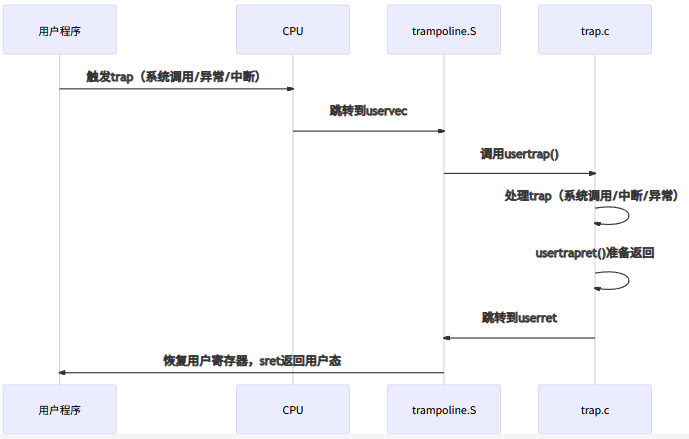
\includegraphics[width=0.4\textwidth]{trap_from_user_space}
	\caption{来自用户空间的内核中断}
	\label{fig:trap_from_user_space}
\end{figure}

\subsection{实验步骤}

\subsubsection{RISC-V 汇编相关问题回答}

阅读 call.asm 中函数 g 、 f 和 main 的代码,回答以下问题:

\begin{enumerate}
	\item 哪些寄存器包含函数的参数?例如,在 main 函数调用 printf 时,哪个寄存器保存的是 13?
	
	答:由\cref{tab:riscv-regs} 所示,a0-a7用于保存函数的参数;在 call.asm 中,找到printf代码,与其相关的汇编指令如\cref{lst:call_printf} 所示,\texttt{24: 4635 li a2,13} 是在地址24的位置,将13加载到\texttt{a2},作为 \texttt{printf} 的第三个参数。
	
	因此,保存 13 的寄存器是 a2。
	
	\item 在 main 函数的汇编代码中,对函数 f 的调用在哪里?对函数 g 的调用又在哪里?(提示:编译器可能会内联函数。)
	
	答:如\cref{lst:call_printf} 所示,\texttt{26:45b1 li a1,12} 是在地址26的位置,将12加载到\texttt{a1},作为 \texttt{printf} 的第二个参数,12 是 \texttt{f(8)+1} 的结果。
	
	说明编译器并没有调用函数 f,而是直接将返回值计算出来了,同样也没有对函数 g 的调用。
	
	\item 函数 printf 位于什么地址?
	
	在 call.asm 中,每个函数开头都有一串十六进制的数字,如 \texttt{000000000000000e <f>:}、\texttt{000000000000001c <main>:} 该数字即为函数的地址。
	
	找到函数 printf 的地址为 0000000000000628。
	
	\item 在 main 中,紧接着 jalr 到 printf 之后,寄存器 ra 中的值是什么?
	
	答:jalr rd, rs1, imm的含义是:rd = PC + 4; PC = rs1 + imm,跳转到PC。\texttt{34: 5f8080e7 jalr 1528(ra)}是跳转到 ra + 1528 的地址,也就是printf的入口,在跳转前会把返回地址(即本条指令的下一条指令的地址)写入 \texttt{ra},以便在执行 \texttt{printf} 后能返回到这里。
	
	因此,寄存器 \texttt{ra} 的值是 34 + 4 = 38。
	
	\item 运行\cref{lst:4_1_5}。输出是什么?输出取决于 RISC-V 是否采用小端模式。如果 RISC-V 采用大端模式,你会将 i 设置为多少才能得到相同的输出? 你需要改变 57616 为不同的值?
	
	答:大端(big-endian)和小端(little-endian)指的是多字节数据类型中哪些字节最重要,并描述字节序列在计算机内存中的存储顺序。在大端系统中,序列中最高有效值存储在最低存储地址(即最前面)。在小端系统中,序列中最低有效值存储在最前面。例如,考虑将 1025(2 的 10 次方加 1)存储在一个 4 字节整数中:00000000 00000000 00000100 00000001。其大端和小端的存储如\cref{fig:big_and_littel_endian} 所示。
	
	许多大型计算机采用大端架构,而大多数现代计算机采用小端架构。
	
	\cref{lst:4_1_5} 的输出结果如\cref{fig:4_1_5_answer} 所示,可以判断运行程序的计算机采用小端模式,如果采用大端模式,需要将 i 改为 0x726c6400,将57616(十六进制为e110)改为286(十六进制为011e)。
	
	\item 在\cref{lst:4_1_6}中, 'y=' ?(注意:答案不是一个具体的值)为什么会这样?
	
	从汇编和底层实现的角度来看,在 RISC-V 架构下,调用 printf 时,前几个参数会被依次放入 a0、a1、a2、a3 等寄存器。例如,printf("x=\%dy=\%d", 3); 实际上传递了两个参数:a0 存放格式字符串 "x=\%dy=\%d",a1 存放整数 3,但没有为第二个 \%d 提供参数(a2 未被初始化)。当 printf 在处理格式字符串时,遇到第一个 \%d,它会从 a1 取出 3 输出;遇到第二个 \%d,它会从 a2 取值,但 a2 里此时可能是上一次函数调用遗留的内容,或者是任意的内存数据,因此输出的 y= 后面会显示一个不可预测的值。这正是因为参数数量和格式化占位符数量不匹配导致的汇编级“脏数据”泄漏到输出中。
	
\end{enumerate}

\begin{listing}[!htb]
	\begin{minted}{c}
#include "kernel/param.h"
#include "kernel/types.h"
#include "kernel/stat.h"
#include "user/user.h"

int g(int x) {
    return x+3;
}

int f(int x) {
    return g(x);
}

void main(void) {
    printf("%d %d\n", f(8)+1, 13);
    exit(0);
}
	\end{minted}
	\caption{call.c源代码}\label{lst:call.c}
\end{listing}

\begin{listing}[!htb]
	\begin{minted}{c}
void main(void) {
    ...
    printf("%d %d\n", f(8)+1, 13);
    24:4635              li a2,13
    26:45b1              li a1,12
    28:00000517          auipc a0,0x0
    2c:7a050513          addi  a0,a0,1952 // 7c8 <malloc+0xe8>
    30:00000097          auipc ra,0x0
    34:5f8080e7          jalr  1528(ra) // 628 <printf>
    ...
	\end{minted}
	\caption{call.asm中与printf代码对应的汇编指令}\label{lst:call_printf}
\end{listing}

\begin{listing}[!htb]
	\begin{minted}{c}
unsigned int i = 0x00646c72;
printf("H%x Wo%s", 57616, &i);
	\end{minted}
	\caption{第(5)问源代码}\label{lst:4_1_5}
\end{listing}

\begin{listing}[!htb]
	\begin{minted}{c}
printf("x=%d y=%d", 3);
	\end{minted}
	\caption{第(6)问源代码}\label{lst:4_1_6}
\end{listing}

\begin{figure}[!htb]
	\centering
	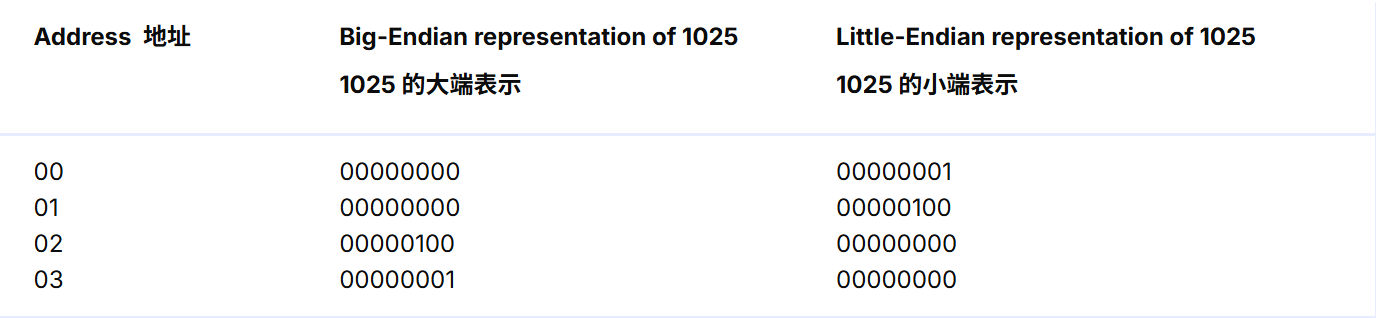
\includegraphics[width=1\textwidth]{big_and_littel_endian}
	\caption{1025在大端和小端的存储方式}
	\label{fig:big_and_littel_endian}
\end{figure}

\begin{figure}[!htb]
	\centering
	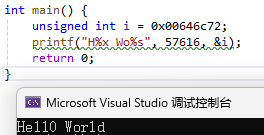
\includegraphics[width=0.6\textwidth]{4_1_5_answer}
	\caption{\cref{lst:4_1_5} 的输出结果}
	\label{fig:4_1_5_answer}
\end{figure}

\subsubsection{实现 Backtrace}

编译器向每一个栈帧中放置一个帧指针(frame pointer)保存调用者帧指针的地址。\texttt{backtrace} 应当使用这些帧指针来遍历栈,并在每个栈帧中打印保存的返回地址。

\begin{enumerate}
	\item 在 kernel/printf.c 中创建函数 \texttt{backtrace},并在kernel/defs.h中声明,在函数 \texttt{sys\_sleep} 中调用。
	\item 将\cref{lst:r_fp} 添加至 kernel/risv.h ,通过 \texttt{uint64 fp = r\_fp()} 读取寄存器 fp 的值。
	\item 根据提示,使用函数 \texttt{PGROUNDDOWN(fp)} 和 \texttt{PGROUNDUP(fp)} 获取堆栈页面的顶部和底部地址,用于终止循环。
	\item 通过 \texttt{uint64 *frame = (uint64*)fp} 将栈顶指针当作指向 8 字节数据的指针。
	\item 由\cref{fig:function_stack_frame}可知,\texttt{frame[-1]} 是函数的返回地址,\texttt{frame[-2]} 是指向上一个栈帧的指针。
	\item 通过循环栈帧指针来遍历堆栈,并在每个栈帧中打印保存的函数返回地址,代码实现如\cref{lst:backtrace} 所示。
	\item 测试 backtrace,成功运行。如 \cref{fig:test_backtrace} 所示
\end{enumerate}

\begin{listing}[!htb]
	\begin{minted}{c}
static inline uint64
r_fp()
{
    uint64 x;
    asm volatile("mv %0, s0" : "=r" (x) );
    return x;
}
	\end{minted}
	\caption{读取寄存器 rp 的值}\label{lst:r_fp}
\end{listing}

\begin{listing}[!htb]
	\begin{minted}{c}
void
backtrace(){
    printf("backtrace:\n");
   
    uint64 fp = r_fp();
    uint64 *frame = (uint64*)fp;
    uint64 up = PGROUNDUP(fp);
    uint64 down = PGROUNDDOWN(fp);

    while(down < fp && fp < up){
        printf("%p\n",frame[-1]);
        fp = frame[-2];
        frame = (uint64*)fp;
    }
}
	\end{minted}
	\caption{函数 backtrace 的实现}\label{lst:backtrace}
\end{listing}

\begin{figure}[!htb]
	\centering
	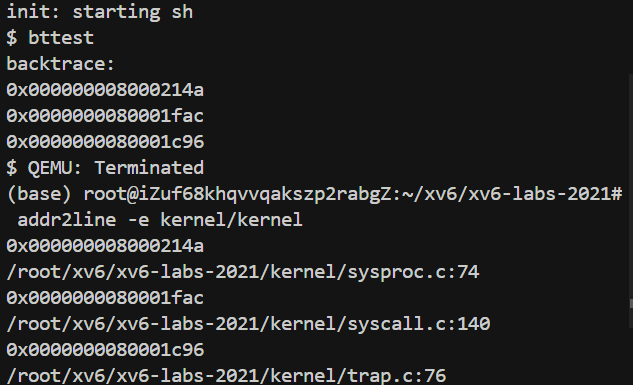
\includegraphics[width=0.6\textwidth]{test_backtrace}
	\caption{测试 backtrace}
	\label{fig:test_backtrace}
\end{figure}

\subsubsection{实现 Alarm}

\paragraph{test0:调用处理程序}

修改内核以跳转到用户空间中的报警处理程序,让 test0 打印 “alarm!”

\begin{enumerate}
    \item 将 \texttt{\$U/\_alarmtest\\} 添加到 Makefile 中
	\item 在 user/user.h 中添加\cref{lst:alarmtest} 声明。
	\item 更新 user/usys.pl、kernel/defs.h、kernel/syscall.h 和 kernel/syscall.c 以允许 alarmtest 调用 sigalarm 和 sigreturn 系统调用。
	\item 暂时将 \texttt{sys\_sigreturn} 的返回值设置为 0。
	\item 在 kernel/proc.h 中,为 \texttt{struct proc} 添加新的变量,如\cref{lst:add_variables_for_proc} 所示。
	\item 在 \texttt{sys\_sigalarm} 中读取参数,将其存储到 \texttt{proc} 的新字段中,如\cref{lst:read_and_write_param} 所示。
	\item 在 kernel/proc.c 中,添加对 \texttt{proc} 新字段的初始化,如\cref{lst:add_alloc_in_allocproc_test0} 和 \cref{add_free_in_freeproc_test0} 所示。
	\item 在 kernel/trap.c 的 \texttt{usertrap} 中,添加对进程的处理,回到用户空间时,能够继续正常执行,如\cref{lst:add_handle_in_usertrap} 所示。
	\item 测试 alarm 的 test0,成功运行,如\cref{fig:test_alarm_test0} 所示。
\end{enumerate}

\begin{listing}[!htb]
	\begin{minted}{c}
int sigalarm(int ticks, void (*handler)());
int sigreturn(void);
	\end{minted}
	\caption{在 user/user.h 中添加 alarmtest 所需函数的声明}\label{lst:alarmtest}
\end{listing}

\begin{listing}[!htb]
	\begin{minted}{c}
struct proc{
    ...
    int ticks;            // 用户设置的周期阈值,每隔多少 tick 触发一次 handler
    int ticks_count;      // 距离上次 handler 触发以来已过去的 tick 数
    uint64 handler;       // 用户注册的信号处理函数的地址(函数指针)
}
	\end{minted}
	\caption{test0 中为 struct proc 添加新的字段}\label{lst:add_variables_for_proc_test0}
\end{listing}

\begin{listing}[!htb]
	\begin{minted}{c}
uint64
sys_sigalarm(void){
    int ticks;
    uint64 handler;
    
    if(argint(0, &ticks) < 0 || argaddr(1,&handler)<0)
        return -1;
    
    struct proc *p = myproc();
    p->ticks = ticks;
    p->handler = handler;
    p->ticks_count = 0;
    
    return 0;
}
	\end{minted}
	\caption{在 sys\_sigalarm 函数中读取参数并存储到 proc 新字段中}\label{lst:read_and_write_param}
\end{listing}

\begin{listing}[!htb]
	\begin{minted}{c}
static struct proc*
allocproc(void){
    ...
    p->ticks = 0;
    return p;
}
	\end{minted}
	\caption{test0 中在 allocproc 函数中添加对 proc 新字段的分配}\label{lst:add_alloc_in_allocproc_test0}
\end{listing}

\begin{listing}[!htb]
	\begin{minted}{c}
static void
freeproc(struct proc *p){
    ...
    p->ticks = 0;
    p->handler = 0;
    p->ticks_count = 0;
}
	\end{minted}
	\caption{test0 中在 freeproc 函数中添加对 proc 新字段的回收}\label{lst:add_free_in_freeproc_test0}
\end{listing}

\begin{listing}[!htb]
	\begin{minted}{c}
void
usertrap(void){
    ...
    if(which_dev == 2){
        if(p->ticks>0){
            p->ticks_count++;
            if(p->ticks_count>p->ticks){
                p->ticks_count = 0;
                p->trapframe->epc = p->handler;
            }
        }
    yield();
    }
}
	\end{minted}
	\caption{在 usertrap 中添加对 proc 新字段的处理}\label{lst:add_handle_in_usertrap}
\end{listing}

\begin{figure}[!htb]
	\centering
	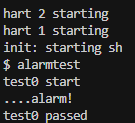
\includegraphics[width=0.3\textwidth]{test_alarm_test0}
	\caption{测试 alarm 的 test0}
	\label{fig:test_alarm_test0}
\end{figure}

\paragraph{test1/test2:恢复被中断的代码}

\begin{enumerate}
	\item 确保完成报警处理程序后返回到用户程序最初被计时器中断的指令执行
	\item 确保寄存器内容恢复到中断时的值,以便用户程序在报警后可以不受干扰地继续运行
	\item 在每次报警计数器关闭后“重新配置”它,以便周期性地调用处理程序。
\end{enumerate}

\begin{enumerate}
	\item 为保存中断时寄存器的内容,并且防止重复调用 \texttt{handler},需要额外在 \texttt{struct proc} 中添加两个字段,如\cref{lst:add_variables_for_proc_test1} 所示。
	\item 在 \texttt{allocproc} 和 \texttt{freeproc} 中设定好相关分配,回收内存的代码,如如\cref{lst:add_alloc_in_allocproc_test1} 和 \cref{lst:add_free_in_freeproc_test1} 所示。
	\item 更新 \texttt{usertrap} 函数,保存进程陷阱帧 \texttt{p$\to$trapframe} 到 \texttt{p$\to$alarm\_trapframe},如\cref{lst:save_trapframe_in_usertrap} 所示。需要注意 \texttt{p$\to$trapframe} 和 \texttt{p$\to$alarm\_trapframe} 都是指针,不能直接复制,而是要拷贝或者迁移。
	\item 在 \texttt{sys\_sigreturn},恢复陷阱帧,如\cref{lst:recover_trapframe_in_sys_sigreturn} 所示。
	\item 测试 alarm 的 test0,成功运行,如\cref{fig:test_alarm_test1_and_test2} 所示。
\end{enumerate}

\begin{listing}[!htb]
	\begin{minted}{c}
struct proc{
    ...
    int is_alarming;                     // 是否正在执行告警处理函数
    struct trapframe *alarm_trapframe;   // 警告陷阱帧
}
	\end{minted}
	\caption{test1 中为 struct proc 添加新的字段}\label{lst:add_variables_for_proc_test1}
\end{listing}

\begin{listing}[!htb]
	\begin{minted}{c}
static struct proc*
allocproc(void){
    ...
    p->ticks = 0;
    return p;
}
	\end{minted}
	\caption{test1/2 中在 allocproc 函数中添加对 proc 新字段的分配}\label{lst:add_alloc_in_allocproc_test1}
\end{listing}

\begin{listing}[!htb]
	\begin{minted}{c}
static void
freeproc(struct proc *p){
    ...
    if(p->alarm_trapframe)
    kfree((void*)p->alarm_trapframe);
    p->alarm_trapframe = 0;
    p->ticks = 0;
    p->handler = 0;
    p->ticks_count = 0;
    p->is_alarming = 0;
}
	\end{minted}
	\caption{test1/2 中在 freeproc 函数中添加对 proc 新字段的回收}\label{lst:add_free_in_freeproc_test1}
\end{listing}

\begin{listing}[!htb]
	\begin{minted}{c}
void
usertrap(void){
    if(which_dev == 2){
        if(p->ticks>0){
            p->ticks_count++;
            if(p->ticks_count > p->ticks && p->is_alarming == 0){
                p->is_alarming = 1;
                memmove(p->alarm_trapframe, p->trapframe, sizeof(struct trapframe));
                p->ticks_count = 0;
                p->trapframe->epc = p->handler;
            }
        }
        yield();
    }
}
	\end{minted}
	\caption{在 usertrap 函数中保存进程陷阱帧}\label{lst:save_trapframe_in_usertrap}
\end{listing}

\begin{listing}[!htb]
	\begin{minted}{c}
uint64
sys_sigreturn(void){
    struct proc *p = myproc();
    memmove(p->trapframe, p->alarm_trapframe , sizeof(struct trapframe));
    p->is_alarming = 0;

    return p->trapframe->a0;
}
	\end{minted}
	\caption{}\label{lst:recover_trapframe_in_sys_sigreturn}
\end{listing}

\begin{figure}[!htb]
	\centering
	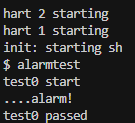
\includegraphics[width=0.3\textwidth]{test_alarm_test0}
	\caption{测试 alarm 的 test1/2}
	\label{fig:test_alarm_test1_and_test2}
\end{figure}

\subsubsection{综合测试}

在 xv6-labs-2021 目录下创建一个time.txt文件,记录我完成该lab花费的时间,再创建一个answers-traps.txt 文件,记录我对 RISC-V 汇编问答题的答案。使用 \texttt{make grade} 对lab4进行综合测试,测试通过。

\begin{figure}[!htb]
	\centering
	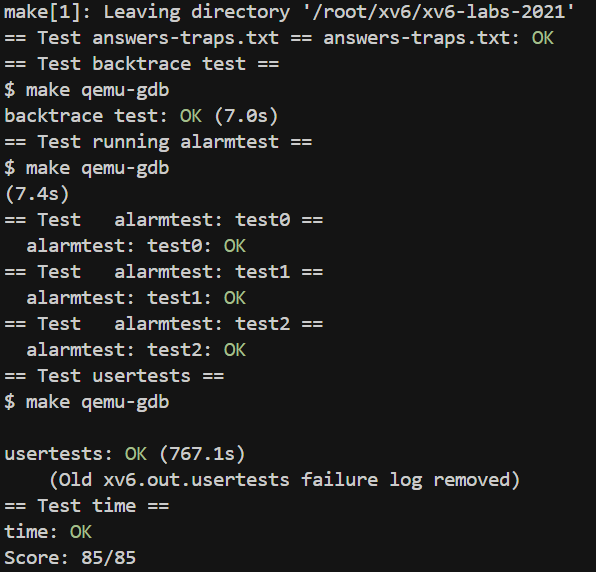
\includegraphics[width=0.5\textwidth]{test_lab4}
	\caption{测试lab4}
	\label{fig:test_lab4}
\end{figure}


\subsection{实验小结}

本次实验通过阅读 xv6 的源码和相关文档,深入理解了系统调用的实现机制,尤其是陷入(trap)和中断的处理流程。通过分析 RISC-V 汇编、栈帧结构以及系统调用的执行过程,我掌握了内核如何通过 trap 机制在用户态和内核态之间切换,并能追踪函数调用栈,定位程序执行路径。通过实现 backtrace 功能,我进一步理解了栈帧指针和返回地址的保存方式,为后续调试和内核开发打下了坚实基础。

在 alarm 部分实验中,我实现了用户级定时中断处理机制,体会到内核如何为用户进程提供定时回调能力。通过设计 sigalarm 和 sigreturn 系统调用,修改 trap 处理流程,并正确保存和恢复用户态寄存器,实现了周期性中断和用户态处理函数的切换。整个过程中,我不仅加深了对操作系统内核时钟中断、进程上下文切换的理解,也锻炼了分析和调试复杂内核问题的能力。